% ══════════════════════════════════════════════════════════════════════════════
%  CHAPTER 8: DARK MATTER
% ══════════════════════════════════════════════════════════════════════════════

\chapter{Dark Matter (Lecture 20-22)}

% =═════════════════════════════════════════════════════════════════════════════
\section{Evidence for Dark Matter}
\begin{intuition}
    Dark matter is a form of matter that does not emit, absorb, or reflect light, making it invisible to electromagnetic observations. Its existence is inferred from its gravitational effects on visible matter, radiation, and the large-scale structure of the universe. \\

    There are multiple lines of evidence for dark matter, including: gravitational lensing, expansion rate of the universe, the CMB anisotropies, and other measurements. We will focus on the most direct evidence for dark matter: galaxy rotation curves, in below sections. We will also briefly discuss an alternative explanation for the observed phenomena: Modified Newtonian Dynamics (MOND).
\end{intuition}

\bigskip \noindent
\begin{extra}
    The name of dark matter was first named d by Jacobus Kapteyn in 1922, he claimed that "dark matter" was not required in galactic Solar neighbourhood. In 1932, Jan Oort suggested that there was twice as much dark matter as luminous matter in the Solar neighbourhood. However, latter observations showed that he was wrong, therefore the discovery of dark matter was credited to Fritz Zwicky who made the first correct claim for the existence of dark matter in 1933. Zwicky concluded from measurements of the redshifts of galaxies in the Coma cluster that their velocities are much larger than the escape velocity due to the visible mass of the cluster. \\

    Between 1950s and 1970s, Vera Rubin and Kent Ford built upon earlier galactic rotation studies and conducted a systematic survey of spiral galaxies.  While their pioneering 1970 paper on the Andromeda galaxy hinted at anomalous outer velocities, it was their work in the mid-to-late 1970s that definitively demonstrated flat rotation curves across many galaxies. These curves showed that stars and gas orbit at nearly constant speeds far beyond the visible disk, rather than declining as expected from luminous matter alone. This systematic evidence firmly established that galaxies are embedded in massive, extended halos of dark matter.
\end{extra}

% ──────────────────────────────────────────────────────────────────────────────
\clearpage
%\bigskip \noindent \bigskip \noindent \bigskip \noindent
\subsection{Galaxy Rotation Curves}
\begin{foundation}
    Start from the Newtonian gravity, the rotational velocity $v$ of a star orbiting at a distance $r$ from the center of a galaxy can be derived from the balance of gravitational force and centripetal force:
    \begin{align*}
        \frac{GM(r)}{r^2} &= \frac{v^2}{r} \\
        v^2 &= \frac{GM(r)}{r}
    \end{align*}
    Then assuming that the mass distribution of the galaxy is concentrated in the center, and density decreases with distance:
    \[
        \rho \propto r^{-n}
    \]
    where $n > 0$, but $n < 3$ to ensure that the total mass is finite. For typical values, $n \approx 2 \sim 3$.

    Now we can get the mass distribution of the galaxy:
    \begin{align*}
        M(r) &= \int_0^r 4\pi r'^2 \rho(r') dr' \\
        &\propto \int_0^r r'^{2-n} dr' \\
        &\propto r^{3-n}
    \end{align*}
    Therefore, the rotational velocity can be derived as:
    \begin{align*}
        v^2 &\propto \frac{r^{3-n}}{r}
    \end{align*}
\end{foundation}

\bigskip \noindent
\begin{theory}
    In newtonian gravity, the rotational velocity $v$ of a star orbiting at a distance $r$ from the center of a galaxy can be expressed as:
    \[
        v = r^{\frac{2-n}{2}}
    \]
    where $n$ is the power-law index of the mass density distribution of the galaxy.
\end{theory}

\clearpage
%\bigskip \noindent
\begin{intuition}
    For $n \approx 2$, we have $v \propto r^0$, which means that the rotational velocity $v$ is constant at large distances from the galaxy center, which is consistent with the observed flat rotation curves. \\
    
    However, from the visible matter distribution, we expect $n > 2$ as stellar density falls rapidly at edges of galaxies, which would predict a declining rotation curve. The conflict between the expected declining rotation curve and the observed flat rotation curve is one of the key pieces of evidence for the existence of dark matter, which provides additional mass that extends beyond the visible matter, leading to a flat rotation curve.
\end{intuition}

\bigskip \noindent
\begin{figure}[htbp]
    \centering
    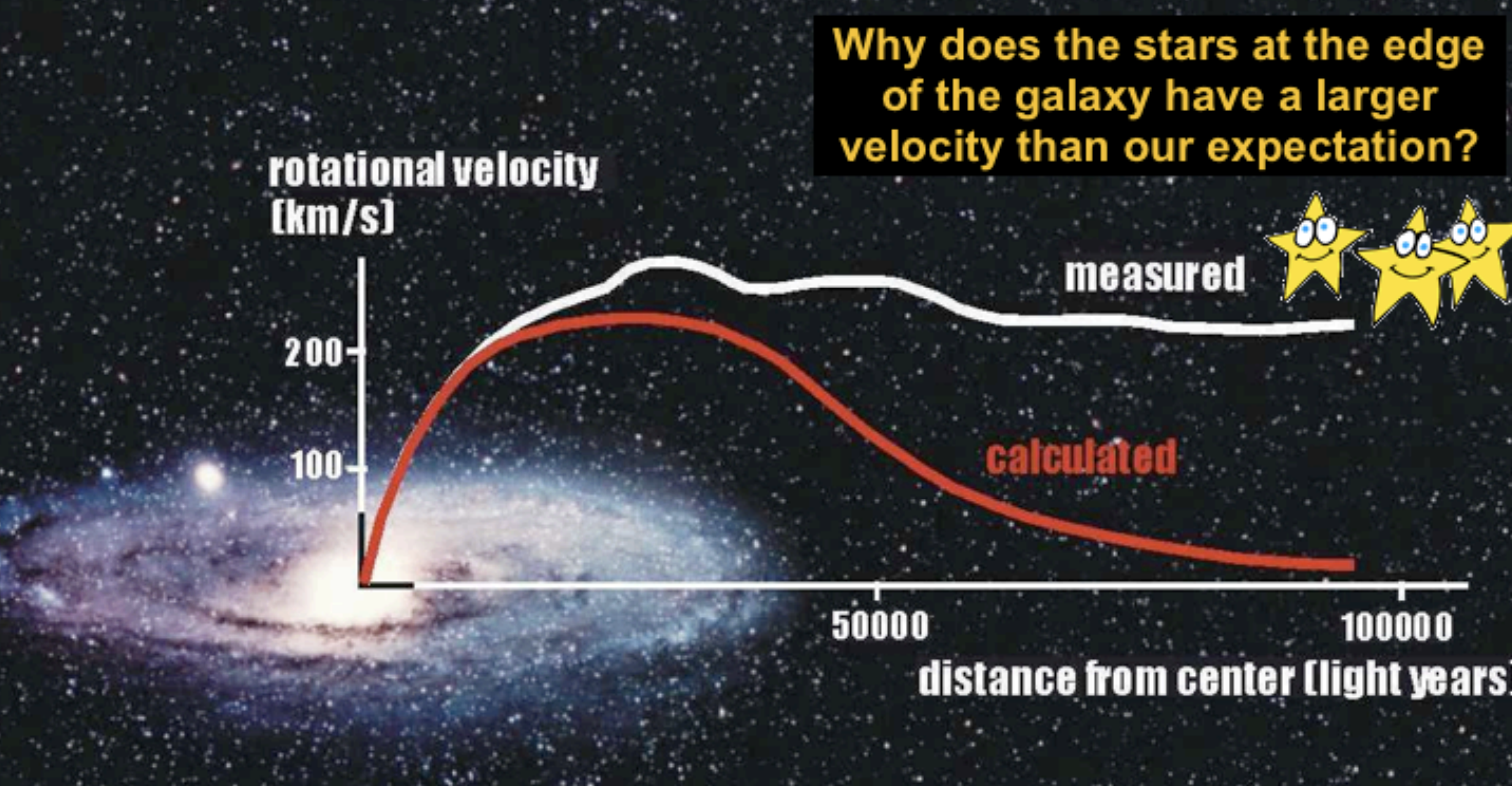
\includegraphics[width=0.8\textwidth]{images/flat_rotation_curves.png}
    \caption{The rotation curve of a galaxy: The red curves represent the expected rotation curve based on the visible matter distribution, which shows a declining trend at large distances. The white curve represents the observed rotation curve, which remains flat at large distances, indicating the presence of dark matter.}
    \label{fig:flat_rotation_curve}
\end{figure}

\begin{extra}
    To describe the observed rotation curves like above figure, the Navarro-Frenk-White (NFW) profile is commonly used to model the dark matter halo of galaxies. The NFW profile is given by:
    \[
        \rho(r) = \frac{\rho_0}{\frac{r}{r_s} \left( 1 + \frac{r}{r_s} \right)^2}
    \]
    where $\rho_0$ is a characteristic density and $r_s$ is a scale radius. The NFW profile predicts a density in 3 parts of the galaxy: 
    (1) Inner region ($r \ll r_s$): $\rho(r) \propto r^{-1}$, which means that density drops but velocity increases as we slightly move away from the center of the galaxy. It matches the rapid increase of the rotation curve in the inner region of the galaxy. \\
    
    (2) Intermediate region ($r \approx r_s$): $\rho(r) \propto r^{-2}$, which means that the density decreases and the velocity remains constant as we move further away from the center of the galaxy. It matches the flat rotation curve in the intermediate region of the galaxy. \\
    
    (3) Outer region ($r \gg r_s$): $\rho(r) \propto r^{-3}$, which means that the density decreases more rapidly and the velocity decreases as we move further away from the center of the galaxy. It matches the declining rotation curve in the outer region of the galaxy.
\end{extra}



% ──────────────────────────────────────────────────────────────────────────────
%\clearpage
\bigskip \noindent \bigskip \noindent \bigskip \noindent
\subsection{Modified Newtonian Dynamics (MOND)}
\begin{intuition}
    Note that existence of dark matter is just a hypothesis to explain the observed phenomena, and there are alternative explanations. One of the most popular alternative explanation is Modified Newtonian Dynamics (MOND), which was proposed by Mordehai Milgrom in 1983. MOND modifies Newton's second law of motion at very low accelerations, which are typically found in the outer regions of galaxies. According to MOND, the effective gravitational force becomes stronger than predicted by Newtonian gravity at these low accelerations, which can explain the flat rotation curves of galaxies without invoking dark matter.
\end{intuition}

\bigskip \noindent
\begin{foundation}
    In MOND, an interpolation function $\mu(a/a_0)$ is introduced too bridge the gap between the Newtonian regime (where $a \gg a_0$) and the MOND regime (where $a \ll a_0$). The modified equation of motion can be written as:
    \begin{align*}
        a \mu \left( \frac{a}{a_0} \right) = a_N = \frac{GM}{r^2}
    \end{align*}
    where $a$ is the actual acceleration, $a_N$ is the Newtonian acceleration, and we required $\mu(x) $ that:
    \begin{align*}
        \mu (x) = \begin{cases}
            1 & \text{for } x \gg 1 \quad \text{(Newtonian regime)} \\
            x & \text{for } x \ll 1 \quad \text{(MOND regime)}
        \end{cases}
    \end{align*}

    A common choice for the interpolation function is:
    \begin{align*}
        \mu(x) = \frac{x}{\sqrt{1+x^2}}
    \end{align*}
    Here we only consider the Deep-MOND regime, where $a \ll a_0$, the equation of motion can be simplified to:
    \begin{align*}
        a \mu \left( \frac{a}{a_0} \right) &= a_N \\
        a \left( \frac{a}{a_0} \right) &= a_N \\
        a^2 &= a_0 a_N \\
        a &= \sqrt{a_0 a_N} \\
        \frac{v^2}{r} &= \sqrt{a_0 \frac{GM}{r^2}} \\
        v^4 &= G M a_0
    \end{align*}
    This result shows that the rotational velocity $v$ becomes constant at large distances from the galaxy center, which is consistent with the observed flat rotation curves.
\end{foundation}

\bigskip \noindent
\begin{theory}
    MOND suggest an modified theory of Newton's laws, with:
    \[
        F = m a \mu \left( \frac{a}{a_0} \right)
    \]
    where $\mu(x)$ is an interpolation function that transitions between the Newtonian regime and the MOND regime, and $a_0$ is a characteristic acceleration scale below which MOND effects become significant, and by galaxy-scale observations, $a_0$ is found to be approximately $1.2 \times 10^{-10} \, \text{m/s}^2$. And we can see that as $a_0$ is extremely small, our labatory experiments are not sensitive enough to detect the MOND effects. \\

    Meanwhile, if scale up to galaxy scale, where the acceleration is much smaller than $a_0$:
    \[
        v = (G M a_0)^{1/4}
    \]
    the rotational velocity $v$ becomes constant at large distances from the galaxy center, which is consistent with the observed flat rotation curves. \\
\end{theory}

\clearpage
%\bigskip \noindent
\begin{intuition}
    While MOND can successfully explain the flat rotation curves of galaxies, it faces 2 main challenges: \\

    (1) Evidence of DM can be found in different physical systems (e.g. galaxy clusters, CMB anisotropies, large scale structure), and if we want to use MOND to explain all these phenomena, gravity must be modified in a more complex way, while the dark matter hypothesis can explain all these phenomena simply. \\

    (It is more related to the principle of Occam's Razor, which states that among competing hypotheses, the one with the fewest assumptions should be selected, another similar case is the geocentric model and the heliocentric model, where the former can explain the observed phenomena by introducing epicycles, while the latter can explain all the phenomena without introducing any epicycle.) \\

    (2) MOND cannot explain the Bullet Cluster, which is a collision of two galaxy clusters. The gravitational lensing observations of the Bullet Cluster show that most of the mass is located in the regions where there is little visible matter, which is consistent with the dark matter hypothesis but cannot be explained by MOND.
\end{intuition}

\bigskip \noindent
\begin{figure}[htbp]
    \centering
    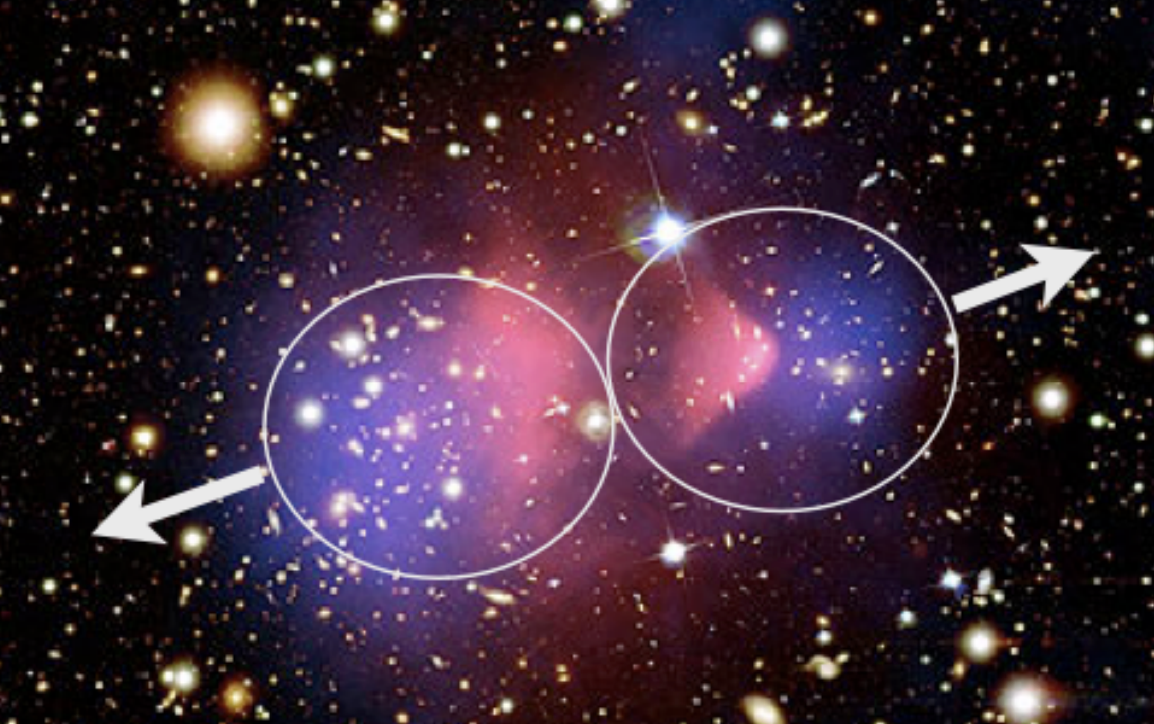
\includegraphics[width=0.8\textwidth]{images/bullet_cluster.png}
    \caption{The Bullet Cluster(NASA, Aug 2006): The blue regions indicate the distribution of dark matter, while the pink regions indicate the distribution of hot gas (which is the dominant form of visible matter in galaxy clusters). The gravitational lensing observations show that most of the mass is located in the blue regions, which is consistent with the dark matter hypothesis but cannot be explained by MOND.}
    \label{fig:bullet_cluster}
\end{figure}

\begin{extra}
    When 2 galaxy clusters collide, if dark matter exist, we will expect to see the hot gas (which is the dominant form of visible matter in galaxy clusters) interacts with each other and slows down, while the dark matter (which does not interact with itself or with visible matter) passes through without slowing down. Therefore, we will expect to see the distribution of dark matter and visible matter are separated. On the other hand, if MOND is correct, we will expect to see the distribution of dark matter and visible matter are the same, because there is no dark matter in MOND. \\
    
    The observations of the Bullet Cluster show that the distribution of dark matter and visible matter are separated, which is consistent with the dark matter hypothesis but cannot be explained by MOND.
\end{extra}









% =═════════════════════════════════════════════════════════════════════════════
\clearpage
%\bigskip \noindent \bigskip \noindent \bigskip \noindent
\section{Properties of Dark Matter}
In the below sub-sections, we will discuss the properties of dark matter in a introduction level.
% ──────────────────────────────────────────────────────────────────────────────
%\clearpage
%\bigskip \noindent \bigskip \noindent \bigskip \noindent
\subsection{Baryonic and Non-baryonic Dark Matter}
\begin{intuition}
    We can classify dark matter into two categories: baryonic and non-baryonic. Baryonic dark matter consists of ordinary matter (protons, neutrons, electrons) that does not emit or absorb significant light, such as MACHOs (Massive Astrophysical Compact Halo Objects), which include black holes, neutron stars, brown dwarfs, and rogue planets. The primary method to detect MACHOs is gravitational microlensing, which occurs when a MACHO passes in front of a background star and temporarily magnifies its light. However, microlensing surveys have detected too few events to account for the total dark matter in galactic halos, indicating that MACHOs can only make up a small fraction of dark matter. \\

    Non-baryonic dark matter candidates, such as WIMPs (Weakly Interacting Massive Particles), axions, and sterile neutrinos, are strongly favored by current observations. Cosmological data from the cosmic microwave background and Big Bang nucleosynthesis show that ordinary baryonic matter accounts for only about 5\% of the universe's total mass-energy budget, while dark matter makes up roughly 27\%, proving that the vast majority of dark matter must be non-baryonic. These candidates are also well-motivated theoretically, as they naturally arise in extensions of the Standard Model of particle physics. Unlike baryonic dark matter in the form of compact objects, non-baryonic dark matter does not produce discrete microlensing events that temporarily brighten background stars. Instead, it exerts a smooth, diffuse gravitational influence, which is fully consistent with observed galactic rotation curves, large-scale structure, and cosmological lensing.
\end{intuition}

\clearpage
\begin{figure}[!htbp]
    \centering
    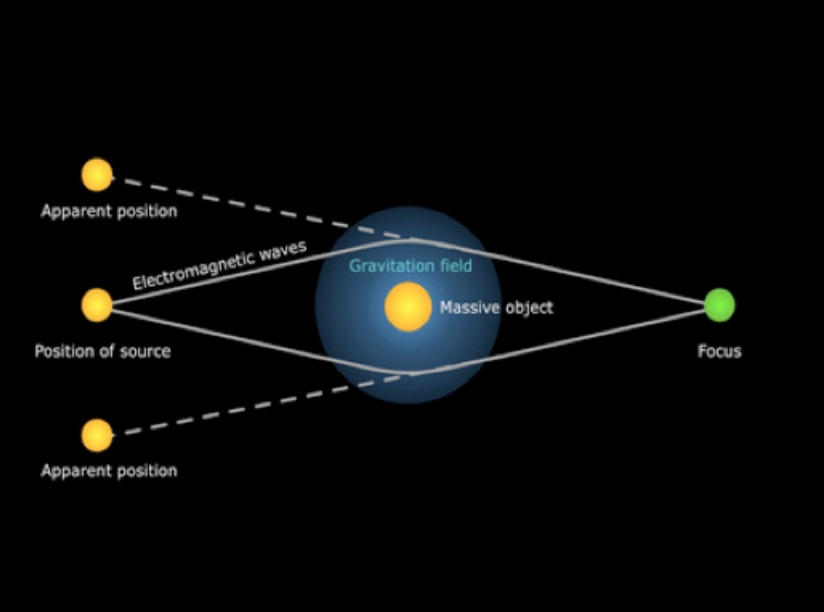
\includegraphics[width=0.6\textwidth]{images/gravitational_microlensing.png}
    \caption{Gravitational microlensing: When a MACHO passes in front of a background star, it can temporarily magnify the light from the star, creating a characteristic light curve. 
    \label{fig:gravitational_microlensing}
    }
\end{figure}

%\bigskip \noindent
\begin{extra}
    In case you have zero knowledge about star evolution, below is a brief introduction of the formation of some objects that can be MACHOs: \\

    (1) Brown Dwarfs: Stars are formed from the gravitational collapse of molecular clouds, and the mass of the collapsing cloud determines the type of star that is formed. If the mass of the collapsing cloud is less than about 0.08 times the mass of the Sun, it will not be able to sustain nuclear fusion in its core, and it will become a brown dwarf. Brown dwarfs are sub-stellar objects that are too massive to be planets but not massive enough to be stars. They emit mainly in the infrared and are very faint, making them difficult to detect. \\

    (2) White Dwarf: when the star reach its end of life, it will collapse under its own gravity, and if the mass of the collapsing part of star is below the Chadrasekhar limit (about 1.4 times the mass of the Sun), it will become a white dwarf. White dwarfs become fade and cool over time, and finally become black dwarfs, which are cold and dark objects that do not emit any light. \\

    (3) Neutron Star: While if the mass of the collapsing part of star is above the Chadrasekhar limit but below the Tolman–Oppenheimer–Volkoff limit (about 2-3 times the mass of the Sun), it will become a neutron star. It is an extremely dense object composed mostly of neutrons, and is super small with only about 10-20 kilometers in diameter. \\

    (4) Black Hole: If the mass of the collapsing part of star is above the Tolman–Oppenheimer–Volkoff limit, it will become a black hole. Black holes are regions of spacetime where gravity is so strong that nothing, not even light, can escape from it. They can be formed from the collapse of massive stars, and they can also be formed from the merger of smaller black holes or from the collapse of dense regions in the early universe.
\end{extra}

% ──────────────────────────────────────────────────────────────────────────────
%\clearpage
\bigskip \noindent \bigskip \noindent \bigskip \noindent
\subsection{Cold and Hot Dark Matter}
\begin{intuition}
    Dark matter is classified based on its velocity distribution (or free-streaming length) at the time of decoupling: cold dark matter (CDM), warm dark matter (WDM), and hot dark matter (HDM). HDM consists of particles that were relativistic at decoupling, typically with very small masses (eV scale or less, like active neutrinos). Their high thermal velocities cause significant free-streaming, which erases small-scale density fluctuations. This would lead to a "top-down" structure formation scenario, where the largest structures form first and later fragment, which is inconsistent with the observed hierarchical, "bottom-up" formation of galaxies and clusters. Consequently, HDM can only constitute a minor fraction of the total dark matter budget. Active neutrinos are the primary example of HDM. \\

    On the other hand, CDM consists of particles that were non-relativistic at decoupling. This category spans a wide mass range: it includes heavy thermal relics like WIMPs (GeV–TeV scale) and extremely light non-thermally produced particles like axions ($\mu$eV–meV scale). CDM's low velocity dispersion allows gravitational collapse on small scales first, driving the bottom-up hierarchical structure formation that precisely matches cosmological observations. The total dark matter density is approximately 27\% of the critical density of the universe, with CDM comprising the dominant component. Current cosmological and astrophysical data strongly favor a CDM-dominated universe.
\end{intuition}

% ──────────────────────────────────────────────────────────────────────────────
\clearpage
%\bigskip \noindent \bigskip \noindent \bigskip \noindent
\subsection{Stableness and Lifetime}
\begin{intuition}
    What makes a particle stable (or sufficiently long-lived)? There are two primary conditions: 
    (1) The particle must carry a conserved quantum number (e.g., electric charge, baryon number, or a discrete symmetry charge like a $Z_2$ parity). 
    (2) It must be the lightest particle carrying that conserved quantity. If a lighter state exists with the same conserved charge, the heavier particle can decay into it while respecting the conservation law. \\

    For example, the electron is absolutely stable because it is the lightest particle with non-zero electric charge. Similarly, the proton is effectively stable because it is the lightest baryon, and baryon number is conserved at the perturbative level in the Standard Model. Conversely, the muon and tau leptons are unstable because they are heavier than the electron and can decay via the weak interaction into lighter leptons while conserving total lepton number. \\
    
    Therefore, if dark matter consists of particles, they must be stable or have lifetimes significantly exceeding the age of the universe ($\tau_{\mathrm{DM}} \gtrsim 10^{17}\,\mathrm{s}$). This typically requires that dark matter particles carry an exactly or approximately conserved quantum number (often imposed via a discrete symmetry) and be the lightest state charged under it, or that their decay channels are highly suppressed by symmetry, large mass scales, or tiny couplings.
\end{intuition}

\bigskip \noindent
\begin{extra}
    The lifetime of other objects as reference:
    \begin{itemize}
        \item Electron: > 4.6 \times 10^{26} \text{ years}
        \item Muon: 2.2 \times 10^{-6} \text{ seconds}
        \item Tau: 2.9 \times 10^{-13} \text{ seconds}
        \item Proton: > 10^{34} \text{ years (current experimental lower limit)}
        \item Age of the universe: \approx 1.38 \times 10^{10} \text{ years}
    \end{itemize}
\end{extra}

% ──────────────────────────────────────────────────────────────────────────────
\clearpage
%\bigskip \noindent \bigskip \noindent \bigskip \noindent
\subsection{Decoupling and Interactions}
\begin{intuition}
    So far, we have known the properties of dark matter as: \\
    (1) It is non-luminous and electrically neutral. \\
    (2) It is non-baryonic and very likely to be a new type of particle that does not exist in the Standard Model. \\
    (3) It is cold (non-relativistic) at the time of decoupling, (i.e. $m_\chi \gg T_{\mathrm{CMB}}$), which means that it has a very small velocity dispersion and can form structures on small scales. \\
    (4) It is stable or has a lifetime much longer than the age of the universe. \\

    Now lets discuss about the interactions and relic abundance of dark matter. 
\end{intuition}

\bigskip \noindent
\begin{intuition}
    If we assume the DM particles remain in thermal equilibrium and never decoupled, then the number density of DM particles would be given by the Maxwell-Boltzmann distribution:
    \[
        n_{\chi,\mathrm{eq}} = g_\chi \left( \frac{m_\chi T}{2\pi} \right)^{3/2} e^{-m_\chi/T}
    \]
    And we will see that the number density of DM particles would be exponentially suppressed at low temperatures, which means that the relic abundance of DM would be negligible. Therefore, we need to consider the case where DM particles decoupled from the thermal bath at some point in the early universe, which allows them to have a non-negligible relic abundance today. \\

    Generally, assumed the stable DM particle $\chi$ is in thermal equilibrium with the Standard Model particles $Y$ in the early universe, and the dominant interaction is $\chi \bar{\chi} \leftrightarrow Y \bar{Y}$. \\
\end{intuition}

\bigskip \noindent
\begin{intuition}
    At the early stage of the universe $T \gg m_\chi$, the process of $\chi \bar{\chi}$ creation and annihilation are in equilibrium, leading $\chi$ to be present in large quantities alongside the various Standard Model particles. \\
    
    As the universe expands and cools down, the temperature drops below the mass of the DM particle ($T < m_\chi$), and the process of $\chi \bar{\chi}$ creation becomes exponentially suppressed due to the Boltzmann factor, while the annihilation process continues to deplete the number of $\chi$ particles. \\
    
    Eventually, when the annihilation rate falls below the expansion rate of the universe (i.e., $\Gamma_{\mathrm{ann}} < H$), the DM particles "freeze out" and their comoving number density becomes constant, leading to a relic abundance that can account for the observed dark matter density today.
\end{intuition}

\begin{example}{ Equation of DM interactions}{}
    Why the equation is $\chi \bar{\chi} \leftrightarrow Y \bar{Y}$, but not $\chi \leftrightarrow Y \bar{Y}$? \\

    \bigskip\textbf{Solution.}\quad \\
    If the process is $\chi \leftrightarrow Y \bar{Y}$, then the DM particle $\chi$ can decay into Standard Model particles $Y$ and $\bar{Y}$, which would violate the stability requirement of dark matter. Since we know that dark matter must be stable or have a lifetime much longer than the age of the universe, the process $\chi \leftrightarrow Y \bar{Y}$ is not allowed. \\
    
    Further, if the process is $\chi \leftrightarrow Y \bar{Y}$, the quantum numbers of $\chi$ must be the same as the combined quantum numbers of $Y$ and $\bar{Y}$, which would require $\chi$ to carry 0 value of the quantum numbers. This also violates the requirement that dark matter must carry a conserved quantum number to ensure its stability.
\end{example}

% ──────────────────────────────────────────────────────────────────────────────
%\clearpage
\bigskip \noindent \bigskip \noindent \bigskip \noindent
\subsection{Boltzmann Equation for DM Relic Abundance}
\begin{foundation}
    Recall the general form of the Boltzmann equation for the number density $n_\chi$ of DM particles:
    \[
        \frac{dn_\chi}{dt} + 3H n_\chi = C[n_\chi]
    \]
    Where LHS actually is the number density conversation equation (you can check chapter 7.3.2 to see how the $3H n_\chi$ term arises), and RHS is the collision term that describes the net effect of annihilation of DM particles. For the process $\chi \bar{\chi} \leftrightarrow Y \bar{Y}$, the collision term can be written as:
    \[
        C[n_\chi] = -\langle \sigma_{\chi \bar{\chi}} v \rangle (n_\chi^2 - n_{\chi,\mathrm{eq}}^2)
    \]
    where $\langle \sigma_{\chi \bar{\chi}} v \rangle$ is the thermally averaged annihilation cross section times velocity, $n_\chi$ is the actual number density of DM particles, and $n_{\chi,\mathrm{eq}}$ is the equilibrium number density of DM particles. The term $n_\chi^2$ represents the annihilation of DM particles, while the term $n_{\chi,\mathrm{eq}}^2$ represents the creation of DM particles from the thermal bath. \\

    On the other words:
    \begin{itemize}
        \item Forward process $\chi \bar{\chi} \to Y \bar{Y}$: the rate is proportional to $n_\chi^2$ because it requires two DM particles to annihilate.
        \item Reverse process $Y \bar{Y} \to \chi \bar{\chi}$: the rate is proportional to $n_{\chi,\mathrm{eq}}^2$ because it depends on the equilibrium abundance of DM particles that can be produced from the thermal bath.
    \end{itemize}

    Now we define the decay rate as:
    \[
        \Gamma_{\chi} = \langle \sigma_{\chi \bar{\chi}} v \rangle n_{\chi,\mathrm{eq}}
    \]
    Substituting the collision term into the Boltzmann equation, we get:
    \begin{align*}
        \frac{dn_\chi}{dt} + 3H n_\chi &= - \langle \sigma_{\chi \bar{\chi}} v \rangle n_{\chi,\mathrm{eq}}^2 \left( \frac{n_\chi^2}{n_{\chi,\mathrm{eq}}^2} - 1 \right) \\
        \frac{dn_\chi}{dt} + 3H n_\chi &= n_{\chi,\mathrm{eq}} \Gamma_\chi \left( 1 - \frac{n_\chi^2}{n_{\chi,\mathrm{eq}}^2} \right)
    \end{align*}
\end{foundation}

\bigskip \noindent
\begin{theory}
    The Boltzmann equation for the number density of DM particles can be written as:
    \begin{align*}
        \frac{dn_\chi}{dt} + 3H n_\chi &= n_{\chi,\mathrm{eq}} \Gamma_\chi \left( 1 - \frac{n_\chi^2}{n_{\chi,\mathrm{eq}}^2} \right) \\
        &= - \langle \sigma_{\chi \bar{\chi}} v \rangle (n_\chi^2 - n_{\chi,\mathrm{eq}}^2)
    \end{align*}
    where $\Gamma_\chi$ is the decay rate of DM particles, $n_\chi$ is the actual number density of DM particles, and $n_{\chi,\mathrm{eq}}$ is the equilibrium number density of DM particles.
\end{theory}
    
\bigskip \noindent
\begin{importantnote}
    Some may confused with the 2 notations $n_\chi$ and $n_{\chi,\mathrm{eq}}$, the former is the actual number density of DM particles, which means the real number density of DM particles we are having in the universe at the given time, and it affects the rate of DM annihilation, because the more DM particles we have, the more likely they will annihilate with each other.

    While the latter is the equilibrium number density of DM particles, which means the number density of DM particles we would have if they were in thermal equilibrium with the thermal bath at the given time. It depends only on current temperature T via statistical mechanics: 
    \[
        n_{\chi,\mathrm{eq}} = g_\chi \left( \frac{m_\chi T}{2\pi} \right)^{3/2} e^{-m_\chi/T}
    \]
    and it affects the rate of DM creation, because it shows the number density of DM particles that can be produced from the thermal bath at the given time.
\end{importantnote}

\bigskip \noindent
\begin{intuition}
     Therefore, at early universe $T \gg m_\chi$, we have $n_{\chi,\mathrm{eq}} \approx n_\chi$, which means rate of DM creation and annihilation are balanced, and DM particles are in thermal equilibrium. \\
    
    As the universe expands and cools down, we have $T < m_\chi$, which means $n_{\chi,\mathrm{eq}} < n_\chi$, the DM particles are no longer in thermal equilibrium, and the annihilation process dominates over the creation process. \\
    
    And at the freeze-out point, we have $\Gamma_\chi = H$, which means the annihilation rate equals the expansion rate of the universe, and $n_{\chi,\mathrm{eq}} \ll n_\chi$, but the expansion of the universe is so fast that the DM particles cannot find each other to annihilate, so the term $n_\chi^2 - n_{\chi,\mathrm{eq}}^2$ is cancel out, which freeze out the number density of DM particles.
\end{intuition}

\bigskip \noindent
\begin{remark}
    In real case, the stage of $n_{\chi,\mathrm{eq}} < n_\chi$ is just short as when $m_\chi < T$, the decay rate $\Gamma_\chi \propto n_{\chi,\mathrm{eq}}$ also drops as $e^{-m_\chi/T}$, which means the 2 conditions nearly happen at the same time, and the freeze-out happens immediately after the DM particles are no longer in thermal equilibrium. So we can treat the intermediate stage and freeze-out stage as the same stage.
\end{remark}


% ──────────────────────────────────────────────────────────────────────────────
%\clearpage
\bigskip \noindent \bigskip \noindent \bigskip \noindent
\subsection{Freeze-out Temperature}
%\bigskip \noindent
\begin{intuition}
    Through the above Boltzmann equation, we can see that the term $\langle \sigma_{\chi \bar{\chi}} v \rangle$ is the key parameter that determines the relic abundance of DM particles. If $\langle \sigma_{\chi \bar{\chi}} v \rangle$ is too large, the DM particles will annihilate too efficiently during the $n_{\chi,\mathrm{eq}} < n_\chi$ stage, leading to a very small relic abundance. \\

    On the other hand, if $\langle \sigma_{\chi \bar{\chi}} v \rangle$ is too small, the DM particles will not annihilate efficiently, and they will freeze out with a large number density, leading to a relic abundance that exceeds the observed dark matter density. \\

    Now lets find out the freeze-out temperature and the relic abundance of DM particles by solving the Boltzmann equation. We will see that if $\langle \sigma_{\chi \bar{\chi}} v \rangle$ is around the weak scale, we can get the correct relic abundance that matches the observed dark matter density, which is known as the WIMP miracle.
\end{intuition}

\bigskip \noindent
\begin{foundation}

\end{foundation}

\bigskip \noindent
\begin{theory}
    The freeze-out temperature $T_{\mathrm{FO}}$ can be expressed as:
    \[
        x_{\mathrm{FO}} \equiv \frac{m_\chi}{T_{\mathrm{FO}}} \approx \ln \left[ c(c+2) \cdot \sqrt{\frac{45}{8}} \frac{g_\chi}{2 \pi^3} \cdot \frac{m_\chi M_{\text{Pl}} \left( a + 6b / x_{\mathrm{FO}}  \right)}{\sqrt{g_*} \cdot \sqrt{x_{\mathrm{FO}}}} \right]
    \]
    with $c \approx 0.5$ is a numerical determined quantity, $g_\chi$ is the number of internal degrees of freedom of the DM particle, $M_{\text{Pl}}$ is the Planck mass, $g_*$ is the effective number of relativistic degrees of freedom at freeze-out, and $a$ and $b$ are the coefficients in the expansion of the thermally averaged annihilation cross section:
    \[
        \langle \sigma_{\chi \bar{\chi}} v \rangle = a + b \langle v^2 \rangle + \mathcal{O}(\langle v^4 \rangle)
    \]
\end{theory}




% ──────────────────────────────────────────────────────────────────────────────
\clearpage
%\bigskip \noindent \bigskip \noindent \bigskip \noindent
\subsection{Relic Abundance}
%\bigskip \noindent
\begin{foundation}
    First, define the comoving abundance of DM particles as:
    \[
        Y_\chi \equiv \frac{n_\chi}{s}  = \frac{n_\text{dec} a^{-3}}{s_\text{dec} a^{-3}} = \frac{n_\text{dec}}{s_\text{dec}}
    \]
    The $Y_\chi$ is the number of DM particles per unit entropy, which is a convenient quantity to use because it remains constant after freeze-out, even as the universe continues to expand and cool down.\\

    and we can rewrite the LHS of the Boltzmann equation as:
    \begin{align*}
        \frac{dn_\chi}{dt} + 3H n_\chi &= s \frac{dY_\chi}{dt} + Y_\chi \frac{ds}{dt} + 3H s Y_\chi 
    \end{align*}
    Note the entropy density $s$ is $propto a^{-3}$, which means $\frac{ds}{dt} = -3H s$, so we have:
    \begin{align*}
        \frac{dn_\chi}{dt} + 3H n_\chi &= s \frac{dY_\chi}{dt} + Y_\chi (-3H s) + 3H s Y_\chi 
        = s \frac{dY_\chi}{dt} 
    \end{align*}

    Similarly, we can rewrite the RHS of the Boltzmann equation as:
    \begin{align*}
        - \langle \sigma_{\chi \bar{\chi}} v \rangle (n_\chi^2 - n_{\chi,\mathrm{eq}}^2) &= - \langle \sigma_{\chi \bar{\chi}} v \rangle s^2 (Y_\chi^2 - Y_{\chi,\mathrm{eq}}^2)
    \end{align*}
    Dividing both sides by $s$, we get:
    \begin{align*}
        \frac{dY_\chi}{dt} &= - \langle \sigma_{\chi \bar{\chi}} v \rangle s (Y_\chi^2 - Y_{\chi,\mathrm{eq}}^2) \\
    \end{align*}

    Now, lets define the inverse temperature variable $x = \frac{m_\chi}{T}$, and:
    \begin{align*}
        \frac{dx}{dt} &= \frac{d}{dt} \left( \frac{m_\chi}{T} \right) \\
        &= - \frac{m_\chi}{T^2} \frac{dT}{dt} \\
        &= - \frac{m_\chi}{T^2} (-H T) \\
        &= H x
    \end{align*}
    which we using the fact that the temperature of the universe scales as $T \propto a^{-1}$, so:
    \begin{align*}
        \frac{dT}{dt} &= \frac{d}{dt}(C a(t)) \\
        & = \frac{C}{a^2} \frac{da}{dt} \\
        & = - \frac{T a}{a^2} \dot{a} \\
        & = - H T
    \end{align*}

    Therefore, we can rewrite the Boltzmann equation as:
    \begin{align*}
        \frac{dY_\chi}{dx} \frac{dx}{dt} &= - \langle \sigma_{\chi \bar{\chi}} v \rangle s (Y_\chi^2 - Y_{\chi,\mathrm{eq}}^2) \\
        \frac{dY_\chi}{dx}  &= \frac{1}{H x} \left( - \langle \sigma_{\chi \bar{\chi}} v \rangle s (Y_\chi^2 - Y_{\chi,\mathrm{eq}}^2) \right) \\
        \frac{dY_\chi}{dx} &= - \frac{\lambda}{x^2} (Y_\chi^2 - Y_{\chi,\mathrm{eq}}^2)
    \end{align*}
    with $\lambda = \frac{s \langle \sigma_{\chi \bar{\chi}} v \rangle}{H} x$. \\

    In fact, we can get details value of $\lambda$ by substituting the expressions of $s$ and $H$:
    \begin{align*}
        \begin{cases}
        s &= \frac{2\pi^2}{45} g_{*s} T^3 \\
        H &= \sqrt{\frac{8\pi G}{3} \rho} = \sqrt{\frac{8\pi G}{3} \frac{\pi^2}{30} g_* T^4}
        \end{cases}
    \end{align*}
    Note here we assume the decoupling happens during the radiation-dominated era, so the energy density $\rho$ and the entropy density $s$ are dominated by the relativistic particles, and we use the relativistic in chpater 5.2 and 5.4 to get the above expressions. \\

    Defining the Planck mass as $M_{\mathrm{Pl}} = \frac{\hbar c}{\sqrt{G}} = \frac{1}{\sqrt{G}} \approx 2.4 \times 10^{18} \, \mathrm{GeV}$, we can rewrite the expression of $\lambda$ as:
    \begin{align*}
        \lambda &= \langle \sigma_{\chi \bar{\chi}} v \rangle \frac{s}{H} x \\
        &= \langle \sigma_{\chi \bar{\chi}} v \rangle \frac{\frac{2\pi^2}{45} g_{*s} T^3}{\sqrt{\frac{8 \pi^3}{90}} \frac{\sqrt{g_*}}{M_{\mathrm{Pl}}} T^2} x \\
        &= \langle \sigma_{\chi \bar{\chi}} v \rangle \left( \frac{2\pi^2}{45} \cdot \sqrt{\frac{90}{8 \pi^3}} \right) \cdot \frac{g_{*s}}{\sqrt{g_*}} \cdot M_{\mathrm{Pl}} \cdot T x\\
        &= \langle \sigma_{\chi \bar{\chi}} v \rangle \left( \sqrt{\frac{\pi}{45}} \right) \cdot \sqrt{g_{*}} \cdot M_{\mathrm{Pl}} \cdot m_\chi
    \end{align*}
    where we take the assumption that $g_{*s} \approx g_*$ in last step, which is valid when there is no significant change in the number of relativistic degrees of freedom around the freeze-out temperature (i.e. before the neutrino decoupling). \\
\end{foundation}

\begin{theory}
    The Boltzmann equation for the comoving abundance can be written as:
    \[
        \frac{dY_\chi}{dx} = - \frac{\lambda}{x^2} (Y_\chi^2 - Y_{\chi,\mathrm{eq}}^2)
    \]
    with $\lambda = \langle \sigma_{\chi \bar{\chi}} v \rangle \left( \sqrt{\frac{\pi}{45}} \right) \cdot \sqrt{g_{*}} \cdot M_{\mathrm{Pl}} \cdot m_\chi$.
\end{theory}

\bigskip \noindent
\begin{foundation}

\end{foundation}

%\bigskip \noindent
\begin{theory}
    The relic abundance of DM particles can be expressed as:
    \[
        \Omega_\chi h^2 \approx 0.1 \left( \frac{x_{\mathrm{FO}}}{20} \right) \left( \frac{g_*}{80} \right)^{-1/2} \left( \frac{a + 3b/x_{\mathrm{FO}}}{3 \times 10^{-26} \, \mathrm{cm}^3/\mathrm{s}} \right)^{-1}
    \]
\end{theory}

\bigskip \noindent
\begin{figure}[!htbp]
    \centering
    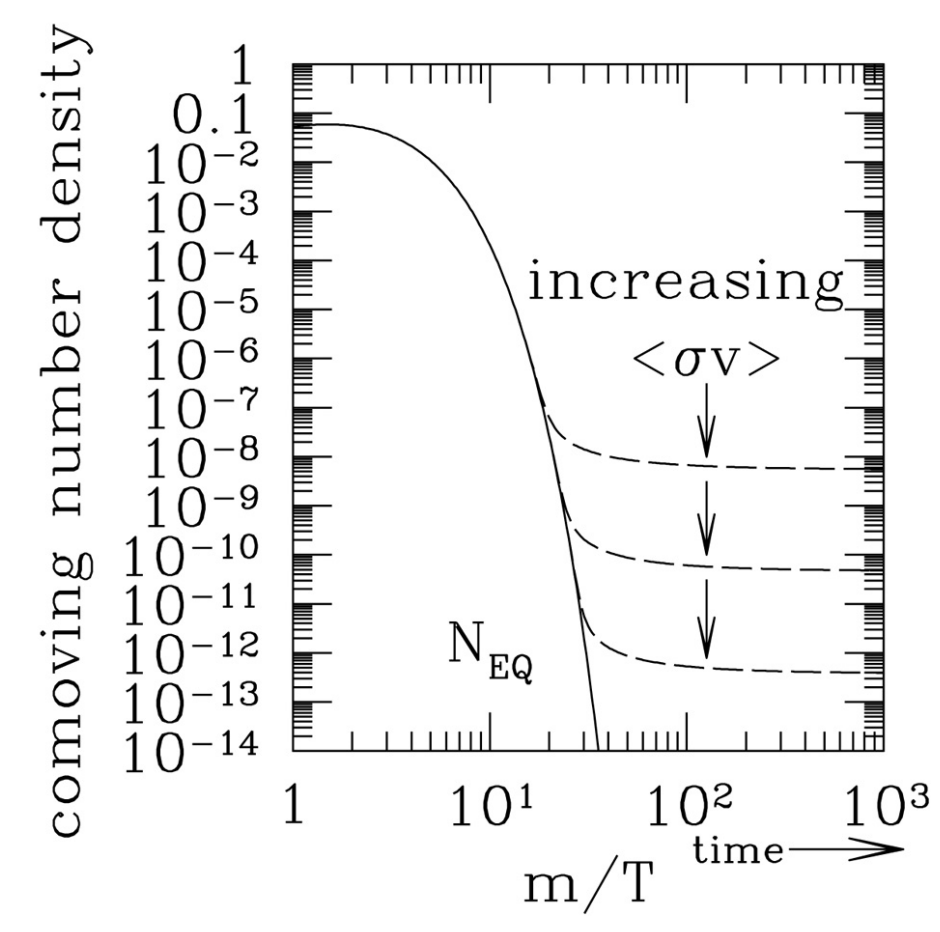
\includegraphics[width=0.7\textwidth]{images/comoving_number_density.png}
    \caption{The evolution of the comoving number density $Y_\chi$ of DM in the freeze-out scenario.}
    \label{fig:comoving_number_density}
\end{figure}

\begin{extra}
    The above figure shows the evolution of the comoving number density $Y_\chi$ of DM particles as a function of the inverse temperature variable $x = m_\chi / T$. The solid line in the figure represents the \textbf{Equilibrium Number Density} $Y_{\chi,\mathrm{eq}}$, while the dashed line represents the \textbf{Actual Number Density} $Y_\chi$. \\

    In the early universe, when $x$ is small, the dashed line closely follows the solid line, indicating that the DM particles are in thermal equilibrium with the thermal bath. As the universe expands and cools down, $T \ll m$ and $x$ increases, and the solid drops exponentially and tends to zero, when new particles cannot be created but remain particles can still annihilate. \\

    However, the dashed line does not drop to zero, and tends to a constant value(i.e. the relic density), the 2 lines separate at the freeze-out point ($m_chi / T \approx 20$), as the free-out stops the annihilation process continues, and the number density of DM particles is frozen at the value at freeze-out, which is much larger than the equilibrium number density at that time. \\

    By the equation we have derived in previous subsection, we know that the cross section $\langle \sigma_{\chi \bar{\chi}} v \rangle$ is also the key parameter that determines the relic abundance of DM particles, it can also be explained by the figure: if $\langle \sigma_{\chi \bar{\chi}} v \rangle$ is small, the particles interact weakly, and they will stop annihilating and freeze out earlier, which means the dashed line will separate from the solid line at a smaller value of $x$, and the relic abundance will be larger. On the other hand, if $\langle \sigma_{\chi \bar{\chi}} v \rangle$ is large, the particles interact strongly, and they will continue to annihilate until a later time, which means the dashed line will separate from the solid line at a larger value of $x$, and the relic abundance will be smaller.
\end{extra}

% ──────────────────────────────────────────────────────────────────────────────
%\clearpage
\bigskip \noindent \bigskip \noindent \bigskip \noindent
\subsection{WIMP Miracle}
\begin{intuition}
    To get the relic abundance that we observed today, we need $\langle \sigma_{\chi \bar{\chi}} v \rangle \approx 3 \times 10^{-26} \, \mathrm{cm}^3/\mathrm{s}$. Interestingly, if we assume the particle is around the weak scale (i.e. $m_\chi \approx 100$~GeV, like W, Z bosons), and it interacts with the weak-force strength (i.e. $\alpha^2 / ( 100 \, \mathrm{GeV} )^2 \approx 10^{-26} \, \mathrm{cm}^3/\mathrm{s}$). This coincidence of alignment between the cosmologic observations and the particle physics scale is known as the WIMP miracle, which makes Weakly Interacting Massive Particles (WIMPs) a very attractive candidate for dark matter. And if the WIMP miracle is true, we should be able to detect WIMPs through their interactions with ordinary matter, which motivates the experimental searches for WIMPs in non-gravitational ways, such as direct detection, indirect detection, and collider detection.
\end{intuition}






% =═════════════════════════════════════════════════════════════════════════════
\clearpage
%\bigskip \noindent \bigskip \noindent \bigskip \noindent
\section{Non-gravitational Detections of Dark Matter}
The "WIMP miracle" shows the DM particles interact with regular matter with a strength comparable to the weak interaction, which means that we can search for DM particles through their non-gravitational interactions with ordinary matter. There are three main methods for non-gravitational detection of dark matter: 
\begin{itemize}
    \item \textbf{Direct Detection}: measuring the interactions between baryonic matter with DM particles.
    \item \textbf{Indirect Detection}: looking for the products of DM annihilation or decay (e.g. gamma rays, neutrinos, cosmic rays) in astrophysical observations.
    \item \textbf{Collider Detection}: searching for the production of DM particles in high-energy particle collisions (e.g. at the Large Hadron Collider), where DM particles would manifest as missing energy and momentum in the detector.
\end{itemize}

\begin{figure}[!htbp]
    \centering
    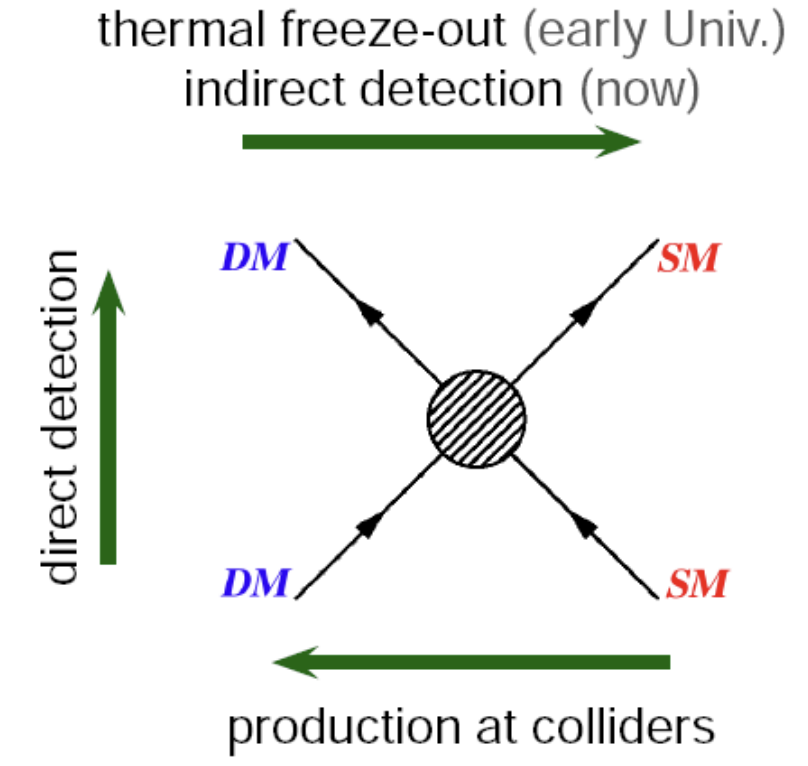
\includegraphics[width=0.55\textwidth]{images/non_gravitational_DM_detection.png}
    \caption{The three main methods for non-gravitational detection of dark matter: direct detection, indirect detection, and collider detection.}
    \label{fig:dark_matter_detection}
\end{figure}

% ──────────────────────────────────────────────────────────────────────────────
\clearpage
%\bigskip \noindent \bigskip \noindent \bigskip \noindent
\subsection{Direct Detection}


% ──────────────────────────────────────────────────────────────────────────────
\clearpage
%\bigskip \noindent \bigskip \noindent \bigskip \noindent
\subsection{Indirect Detection}


% ──────────────────────────────────────────────────────────────────────────────
\clearpage
%\bigskip \noindent \bigskip \noindent \bigskip \noindent
\subsection{Collider Detection}
\begin{intuition}
    Further, we can using a particle accelerator (e.g. LHC in CERN) to create WIMP particle by colliding high-energy particles together. Since WIMPs are weakly interacting and electrically neutral, they would not leave a direct signal in the detector, but we can infer their existence by looking for missing energy and momentum in the collision events. Given that the initial momentum conserved in the \textbf{transverse plane} (perpendicular to the beam axis) is zero:
    \[
        \sum_{\text{vis}} p_{\perp} + \sum_{\text{invis}} p_{\perp} = 0
    \]
    Then, if after collision:
    \[
        \sum_{\text{vis}} p_{\perp} \neq 0
    \]
    i.e. the summation of the transverse momentum of all visible particles is not zero, it indicates that there are invisible particles (e.g. WIMPs) carrying away the missing transverse momentum, which can be a signal for the production of dark matter particles in the collider:
    \[
        \text{Missing Transverse Momentum} = - \sum_{\text{vis}} p_{\perp} = \sum_{\text{invis}} p_{\perp}
    \]
\end{intuition}

\bigskip \noindent
\begin{intuition}
    Some may ask how about using the momentum along the beam axis (i.e. \textbf{longitudinal momentum})? Actually conservation of longitudinal momentum is not useful for detecting WIMPs in collider experiments. \\
    
    In the accelerator, the colliding particles (e.g. protons) are composite particles made up of quarks and gluons, and each of these constituent partons can carry a different fraction of the proton's total momentum. Further, the actual hard collision happens between partons(e.g. gluons and quarks) inside the protons, not the protons themselves \cite{PhysicsGurus_Energies_Accelerator_Collision}, hence:
    \begin{align*}
        \sum_{\text{vis}} p_{\parallel} &\neq 0 \\
        | \sum_{\text{vis}} p_{\parallel} + \sum_{\text{invis}} p_{\parallel} | & \gg 0
    \end{align*}
    As a result, Even we can assume the initial longitudinal momentum of the colliding partons is zero, but we cannot precisely determine the initial longitudinal momentum of the system, and we cant tell the non-zero longitudinal momentum of the visible particles is due to the production of WIMPs or just due to the initial momentum of the partons. Therefore, we focus on the missing transverse momentum, which is well-defined and can be used to infer the presence of invisible particles like WIMPs.
\end{intuition}

\bigskip \noindent
\begin{remark}
    You may ask why the \textbf{transverse momentum} doesn't have the same problem as the \textbf{longitudinal momentum}? Actually, the initial transverse momentum of the colliding partons is effectively zero because the protons are accelerated along the beam axis, and any transverse momentum they have(and their constituent partons have) is negligible compared to the longitudinal momentum. Therefore, any significant missing transverse momentum observed in the detector can be attributed to the production of invisible particles like WIMPs, rather than uncertainties in the initial state of the collision.
\end{remark}

%\bigskip \noindent
\begin{figure}[!htbp]
    \centering
    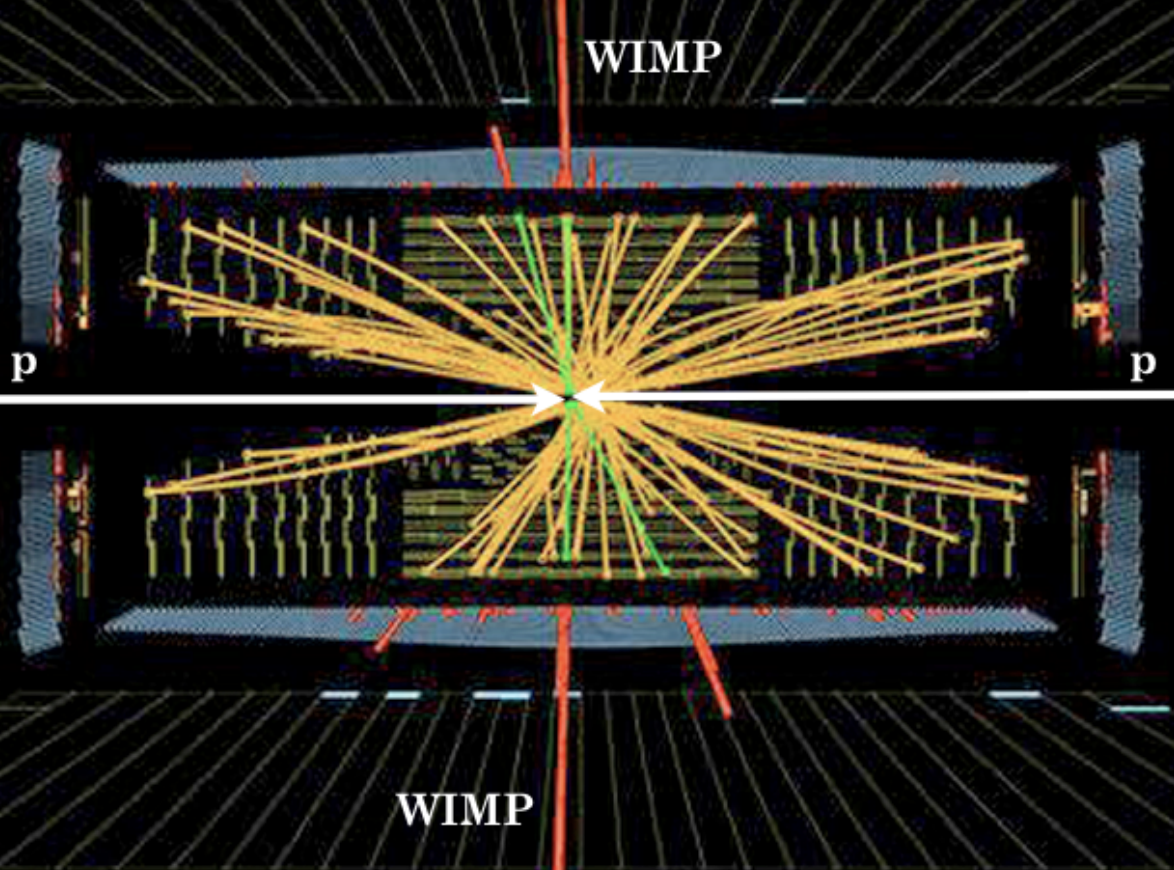
\includegraphics[width=0.7\textwidth]{images/collider_detection.png}
    \caption{A proton-proton collision event in a collider experiment, with potential production of WIMPs (invisible particles) leading to missing transverse momentum.}
    \label{fig:collider_detection}
\end{figure}

\bigskip \noindent
\begin{importantnote}
    However, it is important to note that missing energy signals can also arise from other sources (e.g. neutrinos), so careful analysis and background estimation are required to identify potential dark matter signals in collider experiments.
\end{importantnote}

\bigskip \noindent
\begin{extra}
    In a brief summary, although we have these methods to search for dark matter particles, we have not yet found any conclusive evidence for their existence through non-gravitational interactions. The current search often need combine the results from multiple detection methods (e.g. direct, indirect, and collider) to constrain the properties of dark matter particles and to rule out certain models.
\end{extra}













% =═════════════════════════════════════════════════════════════════════════════
\clearpage
%\bigskip \noindent \bigskip \noindent \bigskip \noindent
\section{Other Candidates for Dark Matter}
As mentioned before, we still don not know what really dark matter is, so except for the WIMP candidates, there are still many hypothetical candidates for dark matter, and we will briefly introduce some of them below. Note that the candidates we will introduce are not exhaustive, and there are many other candidates that are proposed in the literature.
% ──────────────────────────────────────────────────────────────────────────────
%\clearpage
\bigskip \noindent \bigskip \noindent \bigskip \noindent
\subsection{Theoretical Candidates}
%\bigskip \noindent
\begin{figure}[!htbp]
    \centering
    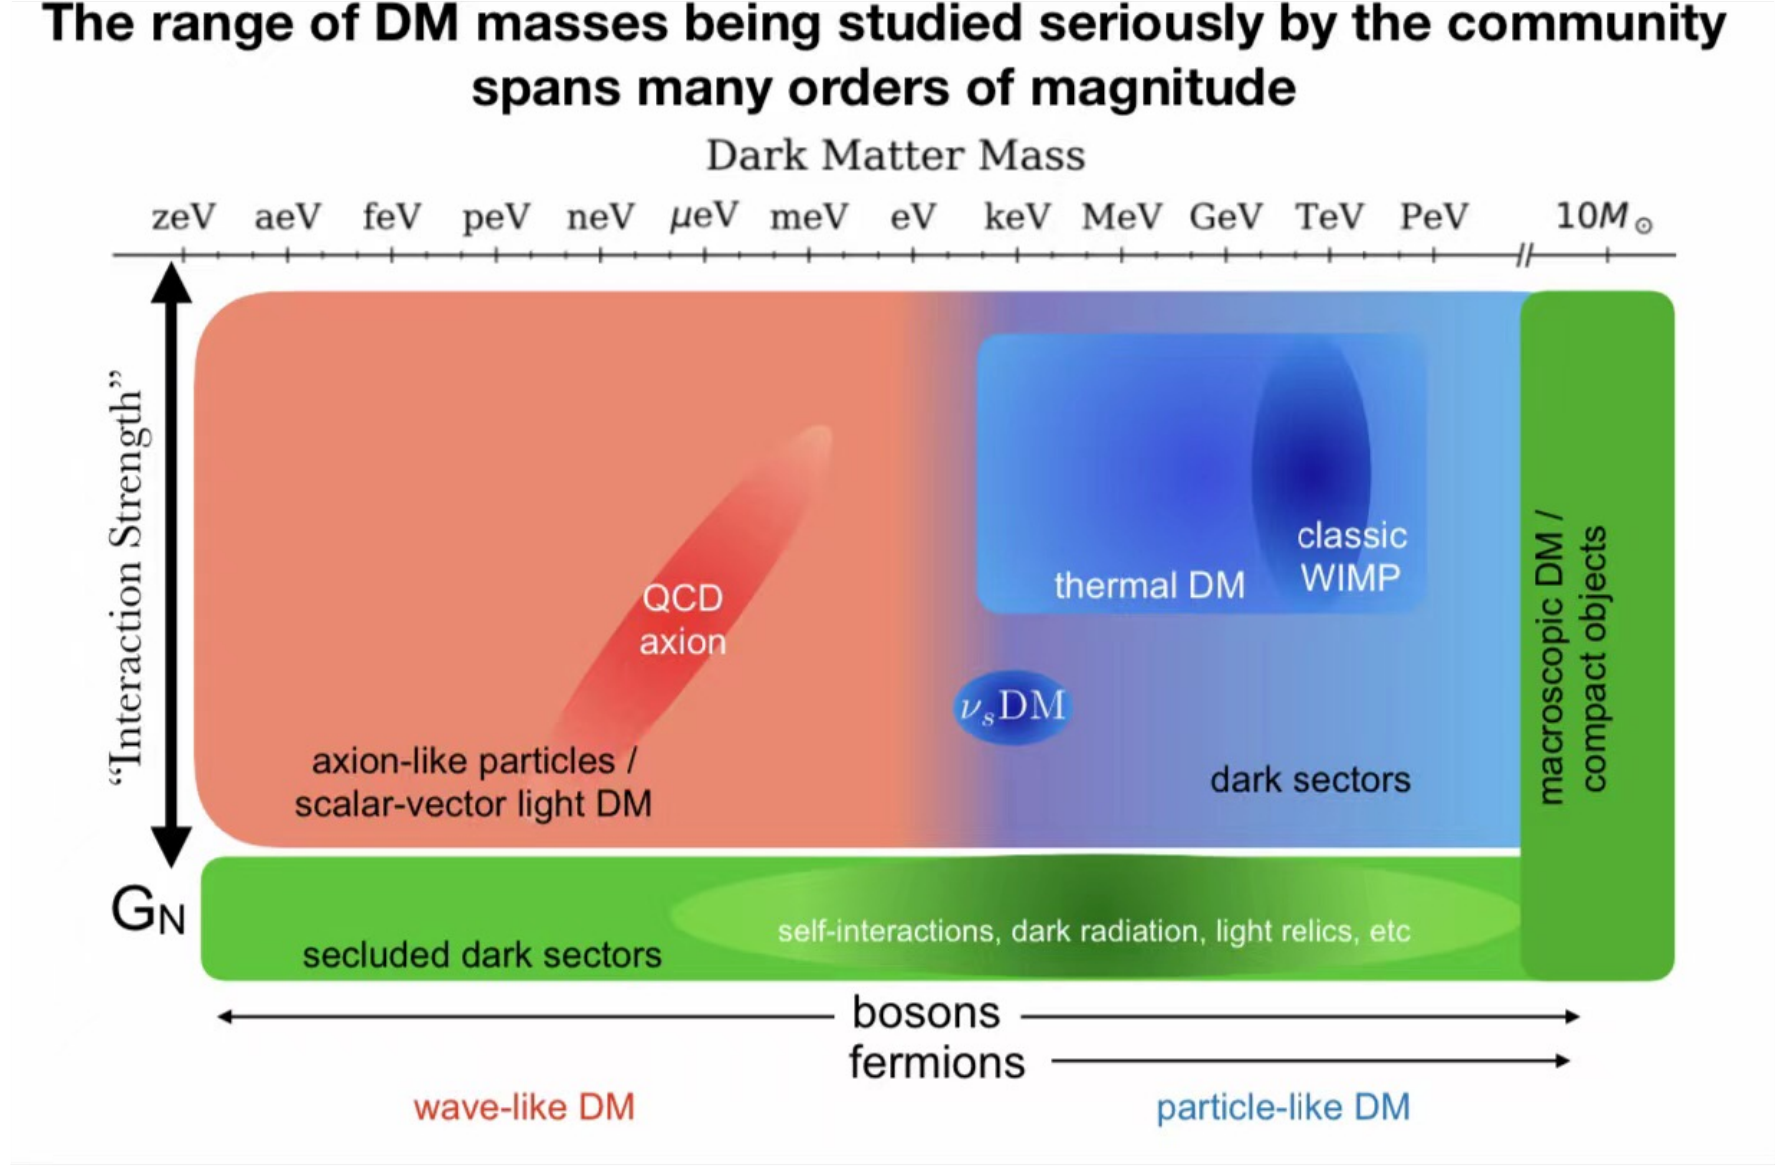
\includegraphics[width=0.85\textwidth]{images/DM_candidates.png}
    \caption{Some of the hypothetical candidates for dark matter.}
    \label{fig:DM_candidates}
\end{figure}

\begin{extra}
    The above figure show some of the hypothetical candidates for dark matter, which x-axis is the mass of the candidate in different energy scale, and y-axis is the interaction strength of the candidate with ordinary matter. The most bottom of y-axis is $G_N$, which means the candidate only interact with ordinary matter through gravity, and when we go up, the particles interact stronger (e.g. via weak nuclear force, or "new dark force"). \\

    We can see that the graph divided into 3 regions, lets start with the \textbf{left region} first, which is the region of Wave-like DM candidates, which are very light particles with very weak interactions. The Paulin exclusion principle prevents these particles from being packed too closely together, so they must be the bosons, and they act like fluid or field and have wave-like properties, they also have very large de Broglie wavelength, which can be comparable to the size of galaxies. Some key candidates in this region include:
    \begin{itemize}
        \item \textbf{QCD Axions}: These are hypothetical particles that arise from the Peccei-Quinn solution to the strong CP problem in quantum chromodynamics (QCD). It locate the transition between the wave-like DM and particle-like DM.
        \item \textbf{Fuzzy DM}: These are ultra-light bosonic particles that behave like oscillating field.
    \end{itemize}
    \\

    The \textbf{right region} is the region of Particle-like DM candidates, which are heavier particles with shorter de Broglie wavelength, and they behave more like distinct particles rather than a fluid. Some key candidates in this region include:
    \begin{itemize}
        \item \textbf{WIMPs}: The classic "Holy Grail" of dark matter candidates, sit in the $GeV$ to $TeV$ mass range, and interact with weak-force strength.
        \item \textbf{Sterile Neutrinos ($\nu_s$ DM )}: A heavier cousin of the known neutrinos, these particles are "warm" dark matter candidates, which means they have a non-negligible velocity dispersion that can affect structure formation on small scales.
    \end{itemize}

    Besides, there is also the \textbf{hidden corners} region (Green regions), it can break to 2 parts: the far right green region is the region of Macroscopic DM/ MACHOs (Massive Compact Halo Objects), which are astrophysical objects that can be made up of ordinary matter but are dark because they do not emit light (e.g. primordial black holes, brown dwarfs, neutron stars, etc.). They are usually massive ($> 1 M_\odot$). \\

    While the bottom green striped region is the region of Secluded Dark Sectors, it is like a "shadow universe" that contains its own particles and forces, they may have their own self-interactions and dark radiation, but they seldom "talk" to our standard model particles, make it hiding in the noise of the universe. As a results, these particles have a wide range of possible masses but only interact with ordinary matter by gravity.
\end{extra}

% ──────────────────────────────────────────────────────────────────────────────
\clearpage
%\bigskip \noindent \bigskip \noindent \bigskip \noindent
\subsection{Primordial Black Holes (PBHs)}
%\bigskip \noindent
\begin{figure}[!htbp]
    \centering
    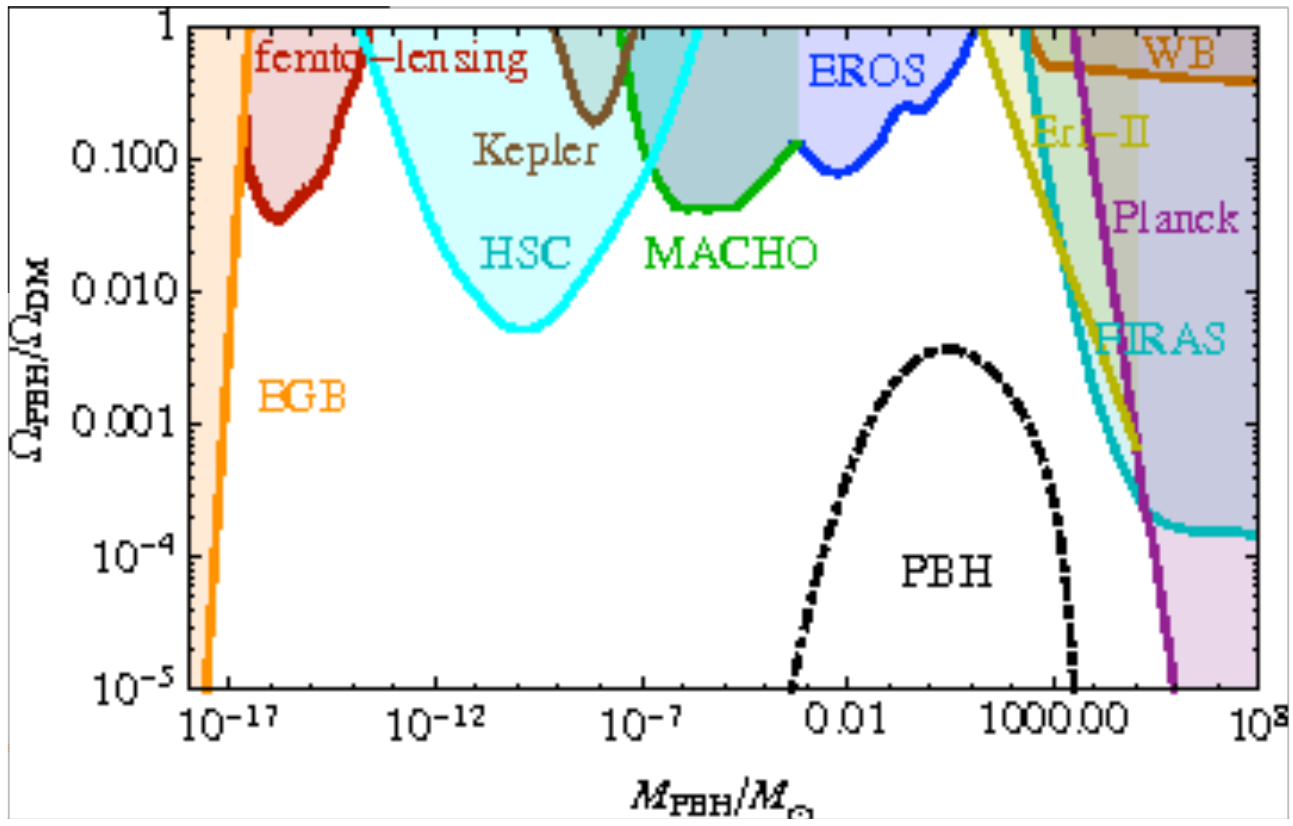
\includegraphics[width=0.7\textwidth]{images/PBH.png}
    \caption{Mass of Primordial Black Holes (PBHs) and corresponding constraints on their abundance as dark matter candidates.}
    \label{fig:PBH_constraints}
\end{figure}

\begin{extra}
    From the above figure, we can see the theoretical fraction of dark matter that can be made up of PBHs(y-axis) against the mass of the PBHs in solar mass(x-axis). While The coloured regions represent the constraints from various observational methods: \\

    \begin{itemize}
        \item \textbf{(1) Microlensing} (Middle "dip" around $10^{-10} M_\odot$):
        \begin{itemize}
            \item intuition: Microlensing occurs when a massive compact object (like a PBH) passes in front of a distant star, causing a temporary increase in the star's brightness due to gravitational lensing. By monitoring the brightness of many stars, we can detect these microlensing events and constrain the abundance of PBHs in certain mass ranges.
            \item constraints: Microlensing surveys (e.g. MACHO, EROS, Kepler, HSC) have placed strong constraints on PBHs in the mass range of approximately $10^{-10} M_\odot$ to $10^{-2} M_\odot$, ruling out PBHs as the dominant component of dark matter in this mass range.
        \end{itemize}
        \item \textbf{(2) Femtolensing \& Evaporation} (Far left):
        \begin{itemize}
            \item intuition: tiny PBHs with masses less than about $10^{-15} M_\odot$ too small to lens stars, but they can still lens high-energy gamma rays from distant sources; while these tiny PBHs can also evaporate via Hawking radiation, producing gamma rays that can be detected by gamma-ray telescopes. If there were enough tiny PBHs, we would expect to see gamma-ray background(i.e. the sky glowing with gamma rays) from their evaporation.
            \item constraints: Femtolensing of gamma-ray bursts and the evaporation detected by Extragalactic Gamma-Ray Background (EGB) measurements can not observed interference patterns or excess gamma rays matching the expected signatures from PBHs, which places strong constraints on PBHs with masses less than about $10^{-15} M_\odot$.
        \end{itemize} 
        \item \textbf{(3) Dynamical Effects \& cosmic Heating}  (Far right):
        \begin{itemize}
            \item intuition: Heavy PBHs with masses greater than about $10^2 M_\odot$ can have significant gravitational effects on their surroundings:
            \begin{itemize}
                \item Cosmic Heating: When heavy PBHs fly around the galaxy (e.g. Eridanus II/ Eri-II), their gravitational interactions can accrete surrounding gas and heat up the gas in the galaxy, which can be observed through X-ray emissions. 
                \item Early Universe Dynamics: If heavy PBHs were abundant in the early universe, their gravitational interactions could heat up the universe and distorting the CMB power spectrum, which can be observed through CMB measurements.
                \item Widely separated binary systems(WB): If heavy PBHs were abundant, they could disrupt widely separated binary systems (e.g. wider binaries in the Milky Way), which can be observed through stellar surveys.
            \end{itemize}
            \item constraints: 
                By looking for the absence of excess X-ray emissions from galaxies such as Eri-II, the lack of distortions in the CMB power spectrum, and the survival of widely separated binary systems, we can place strong constraints on PBHs with masses greater than about $10^2 M_\odot$, ruling out PBHs as the dominant component of dark matter in this mass range.
        \end{itemize}
    \end{itemize}

    Meanwhile, the dashed arch in the middle (around $0.01$ to $1000 M_\odot$) represents the special constraint from the LIGO/Virgo gravitational wave direct detection of binary black hole mergers. If PBHs were abundant in this mass range, we would expect to see a significant number of mergers with masses corresponding to the PBH mass range. However, the observed merger rates and mass distributions from LIGO/Virgo do not match the expected signatures from PBHs, which places additional constraints on PBHs as dark matter candidates in this mass range (i.e. PBHs within this mass range ceiled by the dashed arch and can only make up a small fraction of the total dark matter density). \\

    Still, there is window at around $10^{-13} M_\odot$ to $10^{-14} M_\odot$ where PBHs can potentially make up significant fraction of dark matter $> 10\%$, which is not yet ruled out by current observations.
\end{extra}